\chapter*{\FontH{\Huge Milch und Eis}}
\addcontentsline{toc}{chapter}{Milch und Eis}
\lettrine[lines=3]{\color{DeepPink}H}{och} im Norden, wo es immer Winter ist, liegt das Reich der Königin des Winters, die alle aber Schneekönigin nennen. Sie lebt in einem Palast ganz aus Eis und sogar die Möbel bestehen aus Eis. Wenn im Palast jemand durstig ist, bricht man einfach ein Stück Eis von der Wand ab und wartet bis es im Munde geschmolzen ist.

Von einem Händler aus dem fernen Süden, dem Reich des Königs des Sommers, seinerseits Bademeister gerufen, liess sich die Schneekönigin oft erzählen, wie es in dem warmen Land so zu und her geht.  Eines Tages erzählte der Händler von Tieren, die Kühe genannt werden. Sie erfuhr von Eutern unter deren Bauch, aus denen, wenn man es nur richtig anstellt, eine weisse Flüssigkeit gemolken werden kann, die Milch heisst. Das fand die Schneekönigin aufregend und wollte unbedingt auch einmal ein Glas dieser Milch probieren.

Also schickte sie einen Diener los, der eine solche Kuh in ihr Reich bringen möge. Nach einer langen beschwerlichen Reise konnte der Diener eine Kuh beschaffen. Aber da diese so hoch im Norden nirgends Gras finden konnte und es ihr überhaupt viel zu kalt war, weigerte sie sich, Milch zu geben. Ausserdem war sich niemand im Palast so ganz sicher, was es mit diesem Melken auf sich hatte. Schon nach einer Woche gab die Schneekönigin auf und liess die Kuh zurück zum Reich des Bademeisters bringen.

Der Diener, der dazu beauftragt worden war, erhielt auch gleich noch die Anweisung, ein Glas Milch mitzubringen. Die Schneekönigin konnte zwar keine eigene Kuh halten, der Wunsch Milch zu probieren, war aber geblieben. Als der Diener zurück kam und die Königin endlich einen grossen Schluck nehmen wollte, wurde ihr ganz übel, denn die Milch war auf der langen Reise sauer geworden. Damit hatte niemand gerechnet. Milch war im Reich der Schneekönigin wirklich sehr unbekannt. 
\afterpage{
    \begin{figure}
        \thispagestyle{empty}
        \centering
        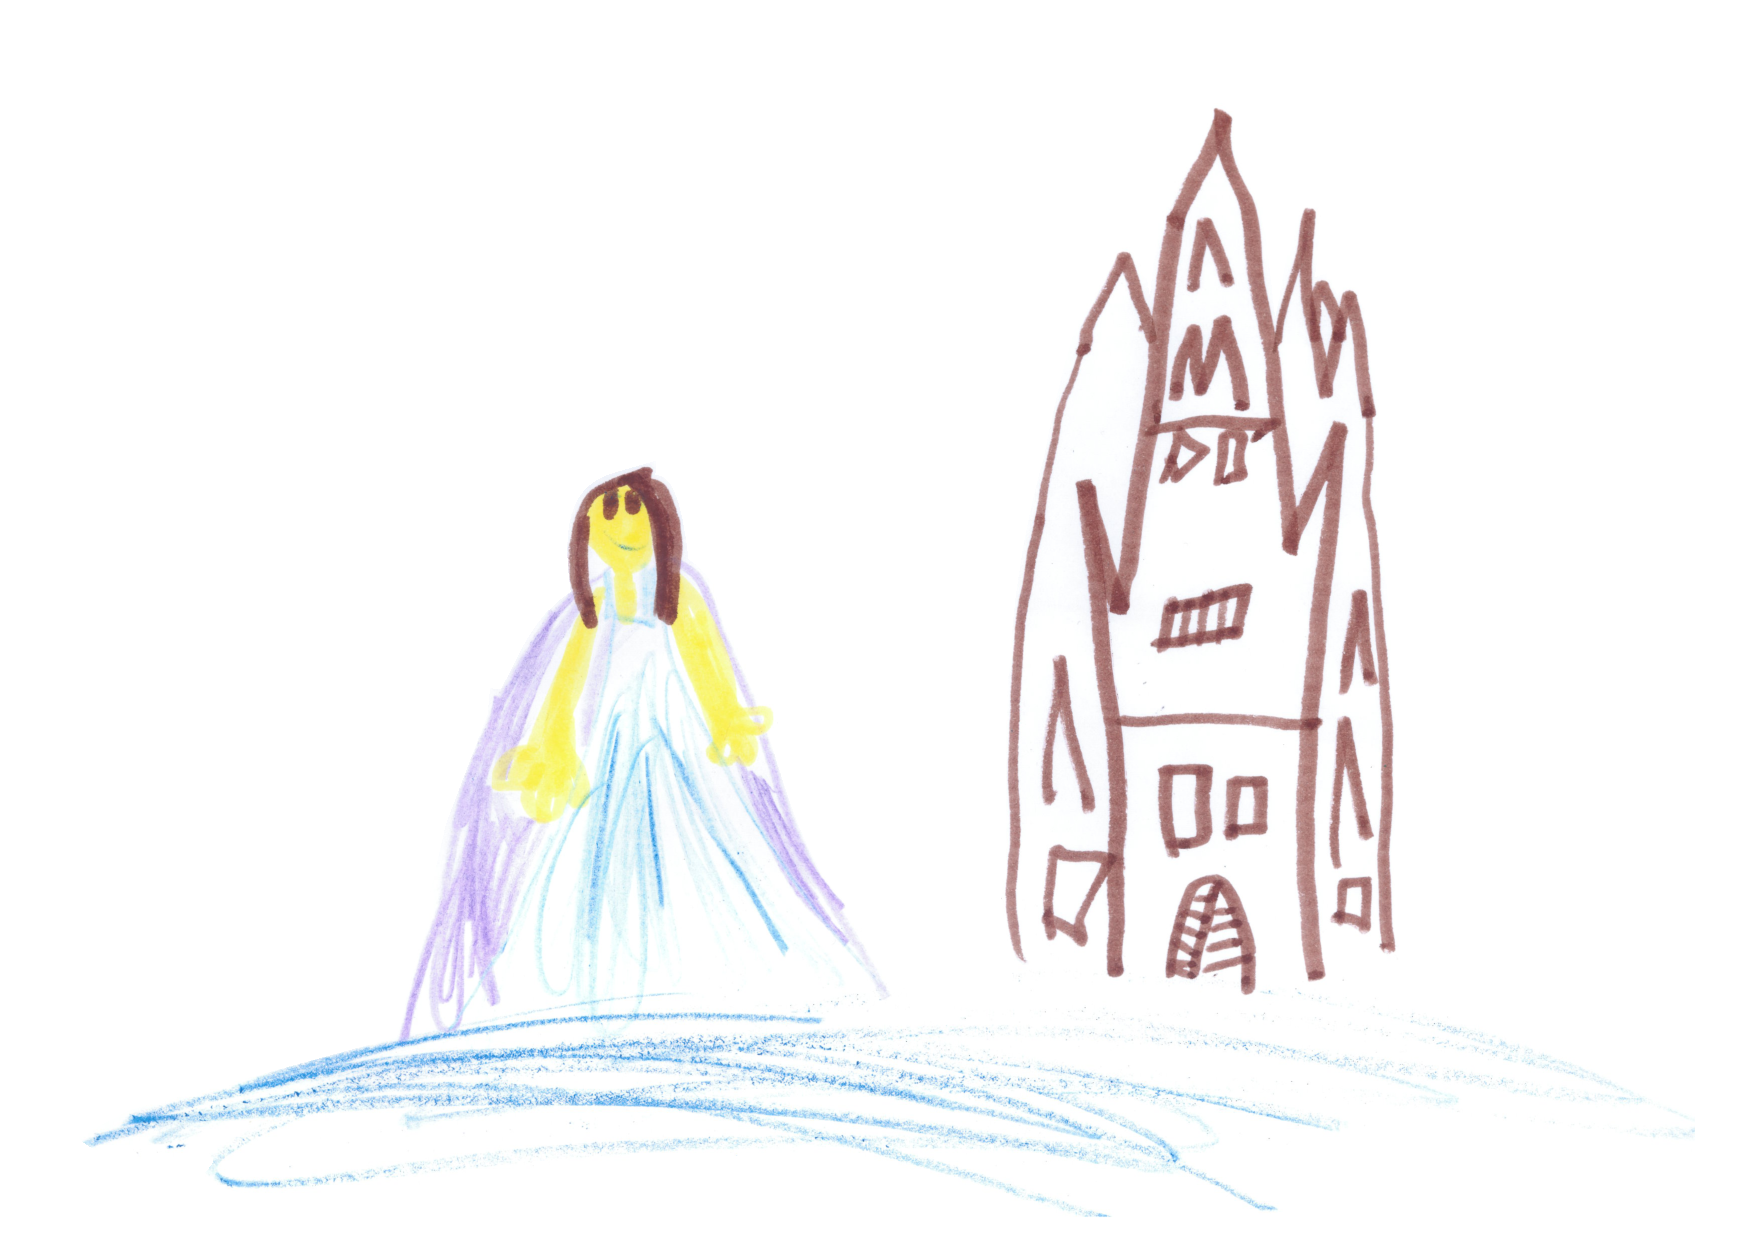
\includegraphics[width=\textwidth]{bilder/schneekoenigin.pdf}       
    \end{figure}
    \clearpage
}

Die weisesten Männer und Frauen des Landes wurden zusammengerufen und sollten Ratschläge erteilen, wie die Milch denn die Reise überstehen könne. Diese wiegten den Kopf hin und her, wer hatte setzte die Brille zurecht und gaben so alle möglichen Tipps. Die Milch müsse mit viel Salz vermischt werden, meinte der eine, nein, man müsse durchgehend rühren, empfahl die andere. 

Aber es war klar, dass eigentlich niemand eine Ahnung hatte. Die Tochter einer Dienerin wusste dann aber doch etwas Überzeugendes, denn die guckte immer die Sendung mit der Maus. Milch, so erklärte sie, werde weniger schnell sauer, wenn man sie nur richtig kühle; im Süden stellen die Menschen sie in Kühlschränke.

Da mussten alle Anwesenden lachen. Das war ja klar, dass die im Süden einen eigenen Schrank haben, der dasselbe schöne Wetter macht, wie sie hier oben tagein, tagaus hatten. Alle fühlten sich bestätigt, dass es hier im Norden ja wohl doch am schönsten, wenn die Bademeisterländer so offen ihren Neid zeigen.

Für solcherlei Diskussionen hatte die Königin keinerlei Sinn. Das sei plumper Nationalismus, entschied sie. Etwas zu kühlen war ganz offensichtlich doch etwas, womit sich die Menschen hier oben wohl am besten auskannten, das musste sie einsehen. 

Die Königin liess einen grossen Klotz Eis herbeischaffen, der in der Mitte einen Hohlraum hatte. Der Eisklotz war so gross, dass wenn er in den Süden und zurück gebracht wurde, zwar beginnen würde zu schmelzen, aber sicher nicht ganz. So blieb die Milch die ganze Zeit von Eis umschlossen und damit kühl. So wurde der Diener wieder auf die Reise geschickt und er konnte einen Bauern finden, der ihm ein Glas voll Milch in den Hohlraum in dem Eisklotz schütten konnte.

Als der Diener mit dem Rest des Eisklotzes wieder bei der Schneekönigin ankam, war aber auch die Milch in seinem Inneren gefroren. Und im Palast war es so kalt, dass sie unmöglich wieder auftauen konnte. Da ja alles aus Eis bestand, waren Wärme und Feuer streng verboten. Enttäuscht liess sich die Schneekönigin auf ihren Thron plumpsen. Der Koch der Königin, ein Italiener namens Gelato war zum Glück ein äusserst raffinierter Vertreter seines Berufes. Er schnitt die gefrorene Milch erst so klein er konnte. Dann zerdrückte er die kleinen Stücke mit der Gabel, um sie dann nochmals kräftig zu rühren, bis eine cremige, kalte Masse entstanden war. In Erinnerung an die saure Milch fügte er zur Sicherheit auch gleich noch etwas Zucker hinzu.

Und das Resultat schmeckte wunderbar. Die Schneekönigin war begeistert und alle, die probieren durften, auch! Noch viel mehr Milch musste in ihren Palast gebracht und zerkleinert und verrührt werden. Schon bald fügte der Koch Gelato noch andere Zutaten seinem Rezept hinzu. Vanille und Schokolade, gefrorene Erdbeeren, Nüsse und Pistazien und was sonst so vom Händler geliefert werden konnte.

Sehr schnell verbreitete sich die Idee Milch zu frieren und zu rühren über die ganze Welt und noch heute nennt man diese feine und kalte Creme in Italien {\itshape gelato} zu Ehren ihres Erfinders.  \hfill {\color{DeepPink}\decofourleft}
